\chapter{Результаты проектирования}

Для хранения узи снимков и кадров используется S3 minio. Структура бакета minio:
\begin{figure}[H]%
	\begin{center}
		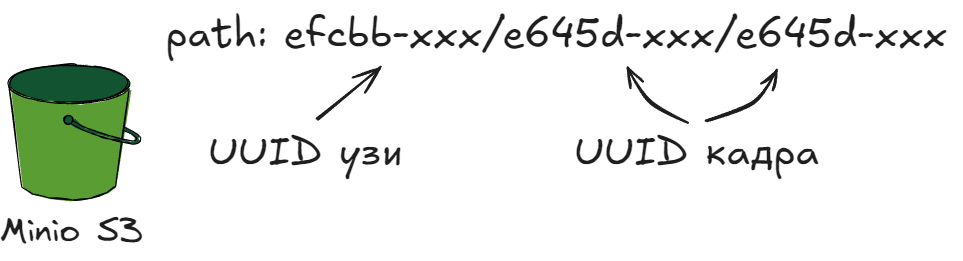
\includegraphics[width=.6\columnwidth]{./img/s3_arc.png}%
	\end{center}
	\caption{Структура S3 хранилища}%
	\label{pic:auth_model}%
\end{figure}

Для использования асинхронного общения через RedPanda, создадим 3 топика:
\begin{itemize}
    \item \textbf{uziupload} - узи загруженно в S3. Запустит разбиение узи на кадры. \ref{lst:uziupload.proto}
    \item \textbf{uzisplitted} - узи разбито на кадры. Запустит обработку узи нейро моделью. В топик пишет Uzi Service после разбиения узи на кадры. \ref{lst:uzisplitted.proto}
    \item \textbf{uziprocessed} - узи обработанно нейромоделью. Узи сегментировано и классифицировано \ref{lst:uziprocessed.proto}
\end{itemize}


\subsection{Auth Service}
\begin{figure}[H]%
	\begin{center}
		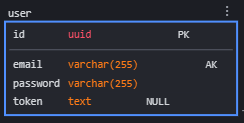
\includegraphics[width=.7\columnwidth]{./img/auth_db.png}%
	\end{center}
	\caption{Спроектированная база данных Auth Service}%
	\label{pic:auth_model}%
\end{figure}


\begin{figure}[H]%
	\begin{center}
		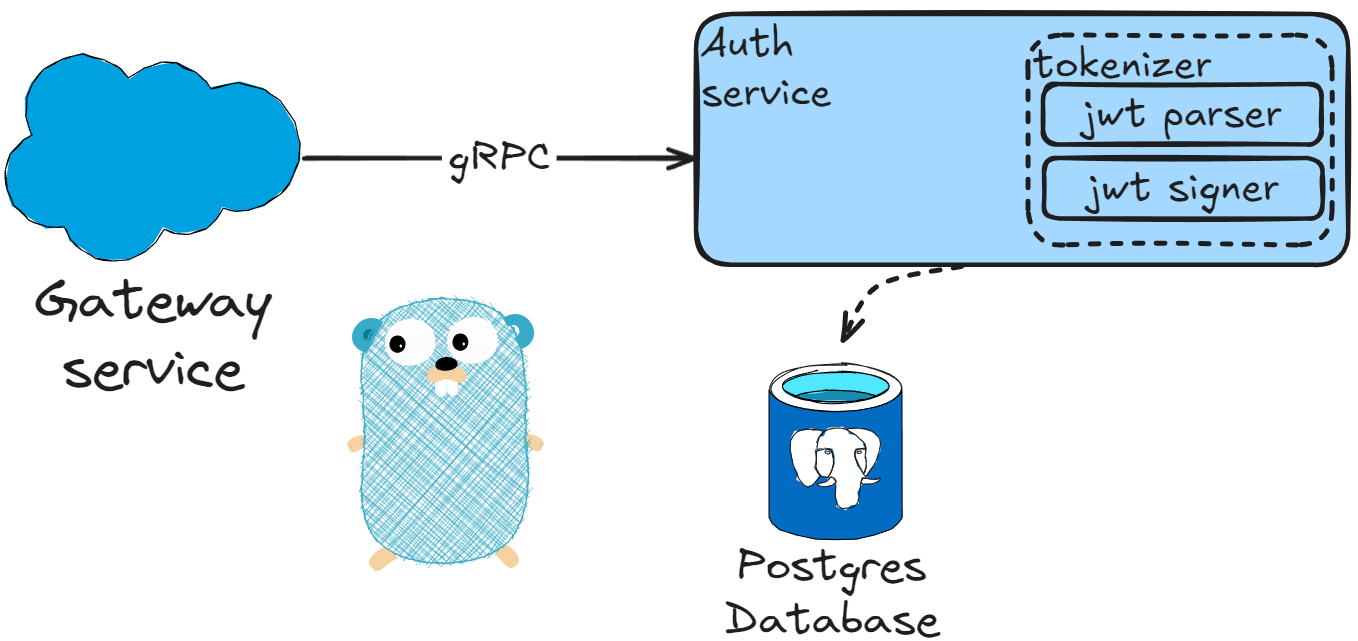
\includegraphics[width=.7\columnwidth]{./img/auth_service.png}%
	\end{center}
	\caption{Auth Service}%
	\label{pic:auth_model}%
\end{figure}

\subsection{Uzi Service}
\begin{figure}[H]%
	\begin{center}
		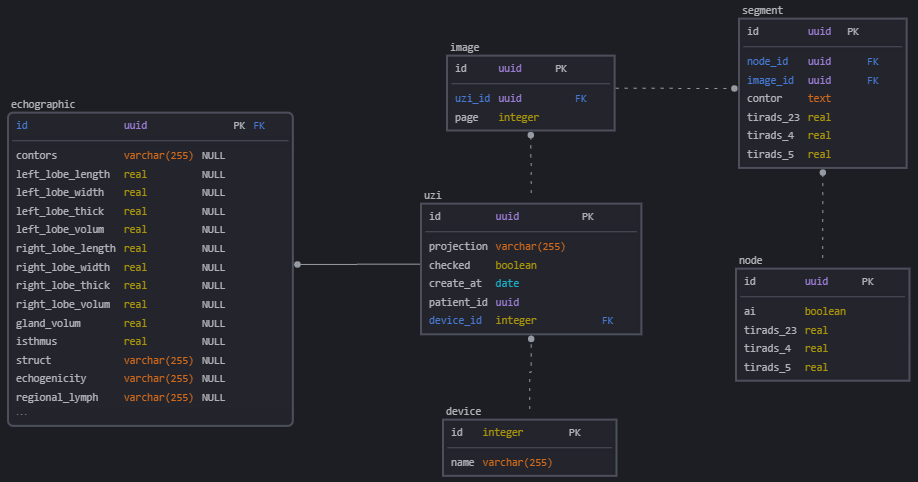
\includegraphics[width=.7\columnwidth]{./img/uzi_db.png}%
	\end{center}
	\caption{Спроектированная база данных Uzi Service}%
	\label{pic:auth_model}%
\end{figure}


\begin{figure}[H]%
	\begin{center}
		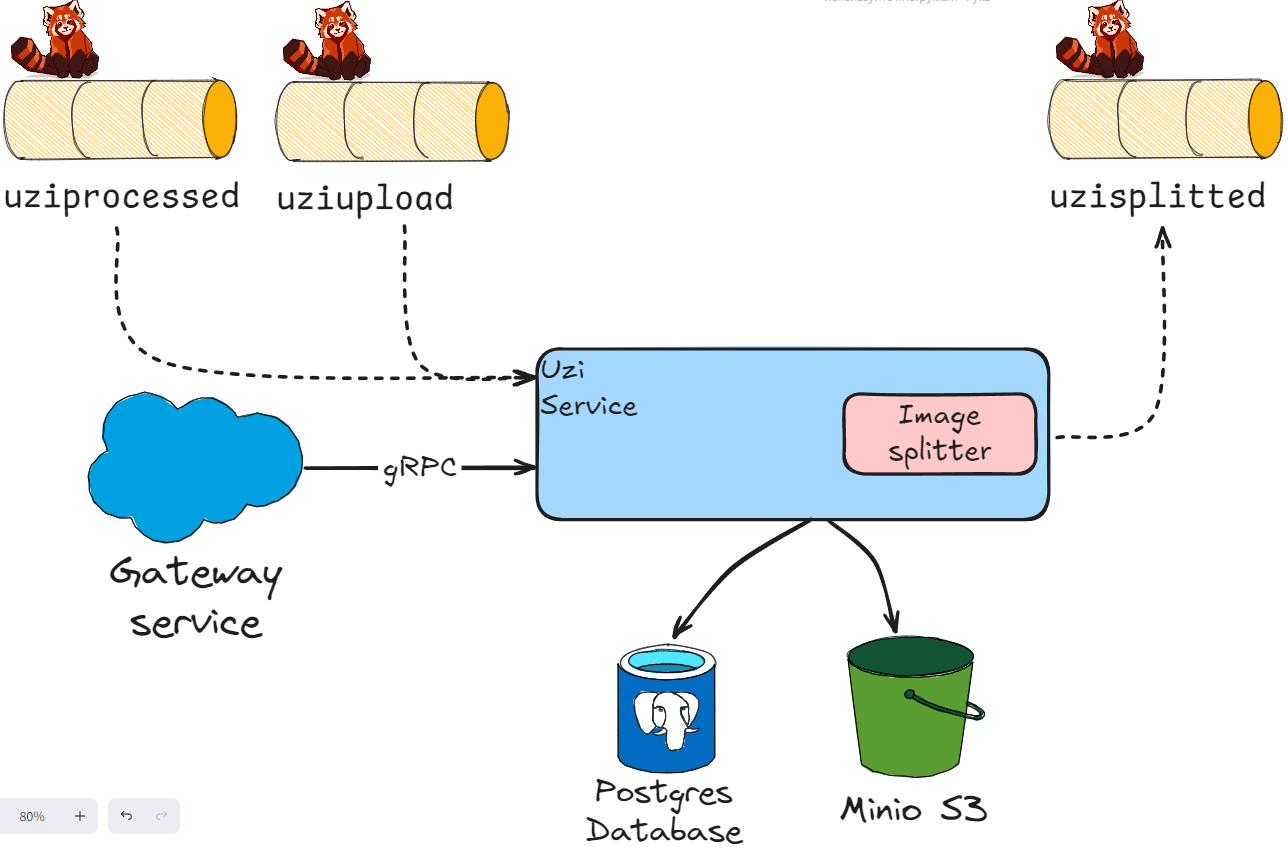
\includegraphics[width=.7\columnwidth]{./img/uzi_service.png}%
	\end{center}
	\caption{Uzi Service}%
	\label{pic:auth_model}%
\end{figure}

\subsection{Gateway API}

\textbf{Распределенные транзакции}
В следствии выбранной микросервисной архитектуры, теряется возможнная атомарность операций, достигаемая
за счет транзакций. Решение этой проблемы реализовано в качестве паттерна Saga. 
С потерей eventual consistency, мы получаем возможнсть производить операцию в транзакции "поэтапно" с возможнстью
откатить все изменения. 

Разберем на примере регистрации нового врача:
\begin{figure}[H]%
	\begin{center}
		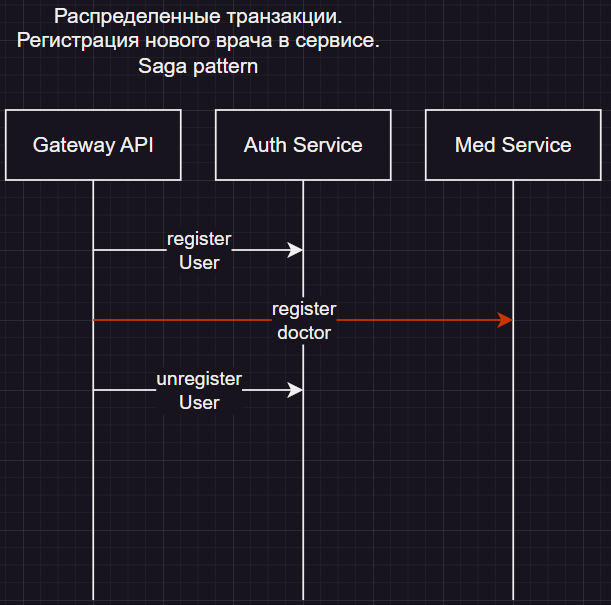
\includegraphics[width=.7\columnwidth]{./img/saga_pattern.png}%
	\end{center}
	\caption{Saga pattern}%
	\label{pic:auth_model}%
\end{figure}


В следующем семестре будет реализованны паттеры transactional outbox и circuit breaker.


\section{Выводы}

В результате были спроектированы модули системы и правила их взаимодействия с учетом выбранных средств разработки
на этапе анализа.
% В этой главе описывается, что и как было спроектировано. 
% При необходимости, описывается использованная методика проектирования. 
% Сюда же относится описание внешних и внутренних программных интерфейсов, 
% а также форматы и структуры входных и выходных данных.


% \section{Использование методики <<такой-то>> для проектирования программных систем <<такого-то типа>>}

% \dots

% \section{Общая архитектура системы \dots}

% \dots


% Команда \texorpdfstring необходима, чтобы программа просмотра PDF документов
% верно отображала текст формул в панели оглавления.
% При отсутствии команды \texorpdfstring там, где она необходима, LaTeX выводит
% предупреждение "Token not allowed in a PDF string"
% \section{Архитектура подсистемы \texorpdfstring{$1$}{1}\dots}

% \dots


% \section{Архитектура подсистемы \texorpdfstring{$N$}{N}\dots}

% \dots


% \section{
%   Проектирование протокола взаимодействия подсистем \texorpdfstring{$X$}{X} и
%   \texorpdfstring{$Y$}{Y}
% }

% \dots


% \section{Выводы}

% Следует перечислить, какие инженерные результаты были получены, а именно: 
% какие программные системы, подсистемы или модули были спроектированы. Следует 
% не только назвать полученные архитектуры, но и отметить их отличительные 
% особенности.

%%% Local Variables:
%%% TeX-engine: xetex
%%% eval: (setq-local TeX-master (concat "../" (seq-find (-cut string-match ".*-3-pz\.tex$" <>) (directory-files ".."))))
%%% End:
